\documentclass[course=asp]{aspdoc}
\usepackage{graphicx}
\graphicspath{{./Bilder/}}

\newcommand{\theGroup}{team 117} % Beispiel: 42
\newcommand{\theNumber}{502: XTEA} 
\author{Guo, Linfeng\\Gönenc, Hazar \\Özakay, Baris}
\date{Wintersemester 2021/22} 


% Diese Zeile bitte -nicht- aendern.
\title{Gruppe \theGroup{} -- Abgabe zu Aufgabe \theNumber}

\begin{document}
\maketitle



\section{Einleitung}
Im Rahmen unseres Projektes im Fach Aspekte der systemnahen Programmierung bei der Spieleentwicklung war es unsere Aufgabe, ein Ver- und Entschlüsselungsalgorithmus XTea in Assemblercode zu programmieren. Diese Aufgabe lässt sich in folgende Bereiche aufteilen: Konzeption, die Funktionsweise des XTEA Algorithmus und Verfahren für die Optimierung des Algorithmus, verstehen; der XTEA Algorithmus in Assemblercode zu implementieren …(Aufgabe von Baris). Die Bearbeitung dieser Teilbereiche wird im Folgenden Beschrieben.  \\In der Grafik zu sehen ist ein Beispiel für die Ver- und Entschlüsselung mit dem XTEA Algorithmus.  

\newpage
\section{Lösungsansatz}
\subsection*{2.1.Feistelchiffre }
Der XTEA Algorithmus ist ein Verschlüsselungsalgorithmus, welche auf die Struktur von Feistelchiffre basiert ist. Feistelchiffre ist eine Struktur, die für symmetrische Verschlüsselung verwendet wird. Unter symmetrische Verschlüsselung ist zu verstehen, dass für die Ver- und Entschlüsselung nur ein Key verwendet wird. Wir würden daher erstmal mit Feistelchiffre, die grundstruktur der symmetrische Verschlüsselung, eingehen.\\
Feistelchiffre lässt sich in vier Schritten aufteilen. Zuerst hat man ein Klartextblock mit der Nachricht, weche meist 8 Bytes ist, und teilt diese in zwei gleich große Bl\"ocke L0 und R0, die 4 Bytes entsprechen auf.

\begin{table}[H]
\centering 
    \begin{tabular}{|l|l|l|l|l|l|l|l|}
        \hline
        B & E & I & S & P & I & E & L   \\
        \hline
    \end{tabular}
    \caption{Nachricht}
\end{table}

\begin{table}[H]
\centering 
    \begin{tabular}{|l|l|l|l|l|l|l|l|}
        \hline
        42 & 45 & 49 & 53 & 50 & 49 & 25 & 4C   \\
        \hline
    \end{tabular}
    \caption{Nachricht in Hex Code}
\end{table}



\begin{table}[H]
    
    \begin{minipage}{.5\linewidth}
      
      \centering
        \begin{tabular}{|l|l|l|l|}
		\hline
            42 & 45 & 49 & 53   \\
		\hline
        \end{tabular}

	\caption{L0}
    \end{minipage}%
    \begin{minipage}{.5\linewidth}
    
 \centering
        
        \begin{tabular}{|l|l|l|l|}
           \hline
		 50 & 49 & 25 & 4C   \\
		\hline
        \end{tabular}
\caption{R0} 
    \end{minipage}
\end{table}
Danach findet die eigentliche Verschlüsselung statt. Man führt die Verschlüsselungsfunktion mit der Schlüssel,der ebenfalls 4 Byte entspricht, auf R0 aus. Die Funktion bei Feistelchiffre ist allerdings undefiniert, da Feistelchiffre nur die Struktur anbietet. Der Wert der durch die Funktion ergibt, wird anschließend mit dem linken Teil durch die XOR- Operation eingefangen. So ergibt sich das neue R1. Die ursprüngliche R0 wird dann zu L1. Nach jeder Verschlüsselung wird die Position vom linken und dem rechten Block getauscht, sowie oben beschrieben wird.\\
Die Entschlüsselung funktioniert im Prinzip genau wie die Verschlüsselung. Nur mit dem Unterschied, dass man die Position vom linken und rechten Teil tauscht. Also wird Ln+1 in die Funktion mit demselben Key eingesetzt und das Ergebnis wird dann mit Rn+1 per XOR abgebildet. Der Wert wird dann zu Rn und Ln+1 wird zu Ln.  

\begin{figure}[h]
\centering
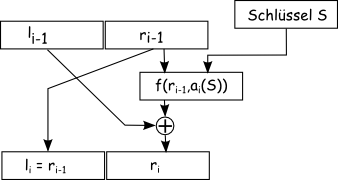
\includegraphics[scale = 0.4]{feistel.png}
\caption{Feistelchiffre}
\end{figure}
\newpage


\subsection*{2.2.XTEA}
Die Aufgabe des Projekts liegt darin den XTEA Algorithmus sowohl in C als auch in Assembler zu implmentieren. Für die Implementierung der XTEA Algorithmus soll man zunächst wissen wie XTEA überhaupt funktioniert. \\
Das Verfahren von XTea ist auf Feistelchiffre basiert. Der eingelesene Wert, welcher 8 Byte entspricht, wird in zwei Blocken aufgeteilt, V1 und V2. Der Schlüssel bei XTEA beträgt 16 Bytes und wird in vier aufgeteilt, die jeweils 4 Bytes entsprichen. Für XTea brauchen wir zusätzlich noch eine weitere Variable s, die Summe, die immer nach der Verschlüsselung Vvon 1 mit der magischen Zahl ${\delta}$ addiert wird. ${\delta}$ lässt sich aus der Formel:
\begin{equation}
     \delta  =   \lfloor ( \surd 5 -1)  \cdot  2^{31} \rfloor
\end{equation}
berechnen. Jede Runde findet eine doppelte Verschlüsselung statt. \\
Zuerst ist die Verschlüsselung von V1. Da wird V2 in zwei Blöcken geshiftet. Block 1: V2 << 4 und Block: V2 >>5. Die zwei Blöcken werden per XOR zu einem neuen Ergebnis abgebildet und mit V2 addiert. Danach wird das Ergebnis mit der Summe von s, welche am Anfang Null ist, und der Schlüssel, dessen Index aus der Variable s Modulo drei ergibt, per XOR abgebildet. Zum Schluss wird das Ergebnis auf V1 addiert. \\
Zur veranschaulichung nehmen wir wieder das Beispielwort "BEISPIEL", in Hex Code. Und teilen dieses Wort in V1 und V2 auf.  
\begin{table}[H]
    
    \begin{minipage}{.5\linewidth}
      
      \centering
        \begin{tabular}{|l|l|l|l|}
		\hline
            42 & 45 & 49 & 53   \\
		\hline
        \end{tabular}

	\caption{V1}
    \end{minipage}%
    \begin{minipage}{.5\linewidth}
    
 \centering
        
        \begin{tabular}{|l|l|l|l|}
           \hline
		 50 & 49 & 25 & 4C   \\
		\hline
        \end{tabular}
\caption{V2} 
    \end{minipage}
\end{table}

\begin{table}[H]
\centering 
    \begin{tabular}{|l|l|l|l||l|l|l|l||l|l|l|l||l|l|l|l|}
        \hline
        41 & 53 & 50 & 41 & 53 & 50 & 41 & 53  & 50 & 41 & 53 & 50 & 41 & 53 & 50 & 41 \\
        \hline
    \end{tabular}
    \caption{Key}
\end{table}

 
Anschließend follgt das Shiften von V2 und die XOR Operation wird danach an den beiden Blöcken ausgeführt.
\begin{table}[H]
    
    \begin{minipage}{.5\linewidth}
      
      \centering
        \begin{tabular}{|l|l|l|l|}
		\hline
            04 & 92 & 54 & C0   \\
		\hline
        \end{tabular}

	\caption{V2 << 4}
    \end{minipage}%
    \begin{minipage}{.5\linewidth}
    
 \centering
        
        \begin{tabular}{|l|l|l|l|}
           \hline
		 02 & 82 & 49 & 2A   \\
		\hline
        \end{tabular}
\caption{V2 >> 5} 
    \end{minipage}
\end{table}

\begin{table}[H]
\centering 
    \begin{tabular}{|l|l|l|l|}
        \hline
        06 & 10 & 1D & EA    \\
        \hline
    \end{tabular}
    \caption{(V2 << 4) $\oplus$ (V2 >> 5)}
\end{table}
Das Ergebnis wird mit V2 addiert. Als nächstes wird die XOR Operation, zwischen dem Ergebnis und der Summe von s und Key, ausgeführt. Da bei der ersten Runde s immer Null ist, wird immer K[0] genommen. 
\begin{table}[H]
\centering 
    \begin{tabular}{|l|l|l|l|}
        \hline
        56 & 59 & 43 & 36    \\
        \hline
    \end{tabular}
    \caption{((V2 << 4) $\oplus$ (V2 >> 5)) + V2}
\end{table}

\begin{table}[H]
\centering 
    \begin{tabular}{|l|l|l|l|}
        \hline
        41 & 53 & 50 & 41    \\
        \hline
    \end{tabular}
    \caption{K[0]}
\end{table}

\begin{table}[H]
\centering 
    \begin{tabular}{|l|l|l|l|}
        \hline
        17 & 0A & 13 & 77    \\
        \hline
    \end{tabular}
    \caption{(((V2 << 4) $\oplus$ (V2 >> 5)) + V2) $\oplus$ (s + K[s\& 3])}
\end{table}
Zum Schluss wird das Ergebnis zu V1 addiert.

\begin{table}[H]
\centering 
    \begin{tabular}{|l|l|l|l|}
        \hline
        59 & 4F & 5C & CA    \\
        \hline
    \end{tabular}
    \caption{((((V2 << 4) $\oplus$ (V2 >> 5)) + V2) $\oplus$ (s + K[s\& 3])) + V1}
\end{table}



Die Variable s wird jetzt um die magische Zahl erhöht. Für V2 funktioniert die Verschlüsselung ähnlich wie bei V1. Wir teilen V1 in zwei Blöcken durch das Shiften auf und genau sowie bei V1, werden die zwei Blöcken per XOR zu einem neuen Ergebnis dargestellt und mit V1 addiert. Das Ergebnis verschlüsselt sich dann per XOR mit der Summe von s und der Schlüssel, dessen Index jetzt aus s shift 11 Modulo 3 besteht. Am Ende wird das Ergebnis auf V1 addiert.
\begin{figure}[h]
\centering
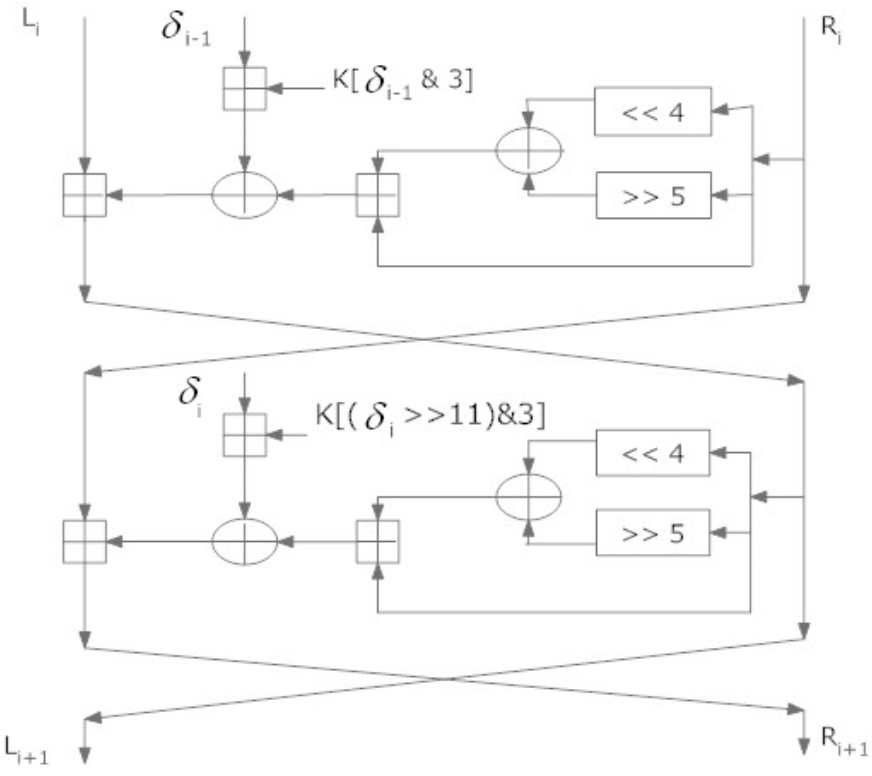
\includegraphics[scale = 0.55]{XTEA.png}
\caption{XTEA(${\delta}$ ist in dem Fall unser s)}
\end{figure}
\newpage




\newpage
\subsection*{2.3.Unterschiede und Gemeinsamkeiten zwischen XTEA und Feistelchiffre}
Die Vorgehensweise beide Verfahren haben Gemeinsamkeiten und Unterschiede. Da XTea auf Feistelchiffre basiert ist, erkennt man auch das symmetrische Verschlüsselungsverfahren bei ihm, d.h. für die Ver- und Entschlüsselung der Nachricht wird denselben Schlüssel verwendet. Bei beidem wird am Anfang der Verschlüsselung die zu verschlüsselnden Daten in zwei Blöcken aufgeteilt und das Verschlüsselungsprozess kann zu mehreren Runden dauern. Die Länge der zu verschlüsselnden Daten muss immer ein Vielfaches der Block-länge sein. Auch das Benutzen von XOR kann man bei beiden Verfahren finden. \\
Es gibt aber auch Unterschiede zwischen beiden Verfahren. Bei XTea findet jede Runde eine doppelte Verschlüsselung statt, was bei Feistelchiffre nicht zu finden ist. Außerdem gibt es bei XTea eine weitere Variable s und die magische Zahl, die bei der Verschlüsselung eine wichtige Rolle spielen. In XTea wird die XOR Operation öfters ausgeführt und zudem verwendet XTea auch das Shiften. Feistelchiffre arbeitet hingegen mit eine Verschlüsselungsfunktion. Nach jedem Runde der Verschlüsselung werden die Position von den zwei Blöcken getauscht, dies kommt bei XTea allerdings nicht vor. \\
Zusammengefasst lässt sich sagen, dass sowohl XTea als auch Feistelchiffre die Voraussetzung für symmetrische Verschlüsselung erfüllen. Bei beidem ist die Länge der zu verschlüsselnden Daten ein Vielfaches der Block-länge. Beide Verfahren teilen die Nachricht für die Verschlüsselung in zwei Blöcken auf, dennoch ist die Key-Schedule bei XTea komplexer ist, im Vergleich zu Feistelchiffre.  

\subsection*{2.4.Verschlüsselung bei Daten die kürzer oder länger als ein Block ist. }
Für Blockverschlüsselungsalgorithmus wie XTea muss die Länge der zu verschlüsselnden Daten immer ein Vielfaches der Block-länge sein. Es kann aber auch manchmal vorkommen, dass die Länge der zu verschlüsselnden Daten länger oder kürzer als 8 Bytes sind. Genau da wird Padding verwendet. Ein Padding Verfahren, das wir für die Implementierung des Algorithmus verwendet haben ist PKCS\#7. PKCS\#7 steht für “Public Key Cryptography Standard” und ist eine Standard-Padding-Methode, die die Zahl der Padding-bytes bestimmen und diese dann als Wert angibt. Unter PKCS\#7 gibt es auch andere PKCS Verfahren, wie zum Beispiel PKCS\#5, welches für die Passwort basierte Kryptographie verwendet wird. PKCS\#7 hingegen ist für sign and/or Verschlüsselung spezialisiert.  \\
Das Padding mit PKCS\#7 funktioniert wie folgt. Angenommen bei einer Blocklänge von 8 Bytes verwenden wir das Wort “ASP”, welche eine Länge von 3 Bytes hat. Das Wort entspricht nicht ein Vielfaches der Block-länge und deshalb wird das PKCS\#7 Verfahren für das Padding verwendet. Die ersten drei Bytes des Blocks sind belegt aber es bleiben noch fünf Bytes offen.  
\begin{table}[H]
\centering 
    \begin{tabular}{|l|l|l|l|l|l|l|l|}
        \hline
        A & S & P & ? & ? & ? & ? & ?    \\
        \hline
    \end{tabular}
    \caption{Nachricht}
\end{table}

\begin{table}[H]
\centering 
    \begin{tabular}{|l|l|l|l|l|l|l|l|}
        \hline
        41 & 53 & 50 & ? & ? & ? & ? & ?    \\
        \hline
    \end{tabular}
    \caption{Nachricht in Hex Code}
\end{table}
Bei PKCS\#7 werden die freien Stellen mit Bytes gefüllt, die jeweils die Anzahl der Füllbytes entsprechen. Also werden in diesem Beispiel die Stellen mit 05 gefüllt.  Die Nachricht kann somit verschlüsselt werden.
\begin{table}[H]
\centering 
    \begin{tabular}{|l|l|l|l|l|l|l|l|}
        \hline
        41 & 53 & 50 & 05 & 05 & 05 & 05 & 05    \\
        \hline
    \end{tabular}
    \caption{Nachricht in Hex Code mit Padding }
\end{table}

Was würde passieren, wenn die zu verschlüsselnde Nachricht länger als ein Block entspricht. Als Beispiel schauen wir uns die folgende Nachricht an “Ich liebe ASP”. Diese Nachricht besteht aus 13 Bytes, länger als ein Block. Daher teilen wir die Nachricht in zwei 8 Bytes Block auf. Die Nachricht in Hex Code umgewandelt sieht wie folgt aus: 
\begin{table}[H]
\centering 
    \begin{tabular}{|l|l|l|l|l|l|l|l|}
        \hline
        49 & 63 & 68 & 20 & 6C & 69 & 65 & 62    \\
        \hline
    \end{tabular}
    \caption{Block 1: Ich lieb}
\end{table}

\begin{table}[H]
\centering 
    \begin{tabular}{|l|l|l|l|l|l|l|l|}
        \hline
         65 & 20 & 41 & 53 & 50 & ?  & ? & ? \\
        \hline
    \end{tabular}
    \caption{Block 2: e ASP}
\end{table}

Jeder 8 Bytes Block wird unabhängig von anderen Blöcken verschlüsselt. Für den ersten Block können wir ohne Probleme verschlüssel. Beim zweiten Block fehlen uns da 3 Bytes. Deshalb verwende wir die PKCS\#7 Methode aus. Hier werden 3 Bytes gefehlt, also füllen wir es mit 03 aus.

\begin{table}[H]
\centering 
    \begin{tabular}{|l|l|l|l|l|l|l|l|}
        \hline
         65 & 20 & 41 & 53 & 50 & 03  & 03 & 03 \\
        \hline
    \end{tabular}
    \caption{Block 2: e ASP mit Padding}
\end{table}
So kann jetzt Block 2 auch ohne Probleme verschlüsselt werden.\\
Zusammengefasst lässt sich sagen, wenn die zu verschlüsselden Daten kürzer als ein Block ist, werden zu nächst das Padding angewendet und danach verschlüsselt. Wenn die Daten jedoch länger als ein Block entspricht, werden die Daten in mehrere Blocks aufgeteilt, jeweils 8 Bytes pro Block. Die Blocks werden unabhängig von einander verschlüsselt. Wenn ein Block nicht mit 8 Bytes voll gefüllt wird, wird es zuerst Padding verwendet und dann verschlüsselt.


%%test
\newpage
% TODO: Je nach Aufgabenstellung einen der Begriffe wählen
\section{Korrektheit/Genauigkeit}
\subsection*{I/O-Operationen in C}
\subsection*{Implementierung in C}
\subsection*{Implementierung in Assemblercode}
\newpage

\section{Performanzanalyse}
\begin{table}[H]
\centering 
    \begin{tabular}{|l|l|l|l|l|l|l|}
        \hline 65 & 20 & 41 & 53 & 50 & 03  & 03  \\
        \hline 65 & 20 & 41 & 53 & 50 & 03  & 03  \\
	\hline 65 & 20 & 41 & 53 & 50 & 03  & 03  \\
	\hline 65 & 20 & 41 & 53 & 50 & 03  & 03  \\
	\hline 65 & 20 & 41 & 53 & 50 & 03  & 03  \\
        \hline 65 & 20 & 41 & 53 & 50 & 03  & 03  \\
	\hline 65 & 20 & 41 & 53 & 50 & 03  & 03  \\
	\hline 65 & 20 & 41 & 53 & 50 & 03  & 03  \\
	\hline 65 & 20 & 41 & 53 & 50 & 03  & 03  \\
        \hline 65 & 20 & 41 & 53 & 50 & 03  & 03  \\
	\hline 65 & 20 & 41 & 53 & 50 & 03  & 03  \\
	\hline 65 & 20 & 41 & 53 & 50 & 03  & 03  \\
	\hline 65 & 20 & 41 & 53 & 50 & 03  & 03  \\
        \hline 65 & 20 & 41 & 53 & 50 & 03  & 03  \\
	\hline
    \end{tabular}
    \caption{Block 2: e ASP mit Padding}
\end{table}
\newpage

\section{Zusammenfassung und Ausblick}

\newpage
% TODO: Fuegen Sie Ihre Quellen der Datei Ausarbeitung.bib hinzu
% Referenzieren Sie diese dann mit \cite{}.
% Beispiel: CR2 ist ein Register der x86-Architektur~\cite{intel2017man}.

%%TODO
\bibliographystyle{plain}
\bibliography{Ausarbeitung}{}

\end{document}
